\newpage
%\pagestyle{empty}

\begin{minipage}[c]{.25\linewidth}
	
\includegraphics[width=4cm]{images/Logo-LEnsE.png}
\end{minipage} \hfill
\begin{minipage}[c]{.4\linewidth}

\begin{center}
\vspace{0.3cm}
{\Large \textsc{Interféromètre de ZYGO}}

\medskip

\textbf{\Large \textsc{Mesure de la phase}}

\end{center}
\end{minipage}\hfill

%%%%%%%%%%%%%%%%%%%%%%%%%%%%%%%%%%
\section{Principe de la mesure de la phase}

En interférométrie, l'intensité enregistrée à un point donné dépend de la différence de phase entre deux ondes lumineuses. Pour retrouver cette phase, on modifie intentionnellement la phase d'une des ondes (typiquement à l'aide d'un miroir piézoélectrique), ce qu'on appelle un décalage de phase (\textit{phase shift}), et on enregistre plusieurs images pour reconstituer la phase locale.

L'intensité mesurée en un point est donnée par :

$$I_k = I_0 + I_1 \cdot cos(\Phi + \delta_k)$$

où $I_0$ est l'intensité moyenne,$I_1$ est le contraste, $\Phi$ est la phase que l'on cherche à déterminer et $\delta_k$ est le décalage appliqué à l'étape $k$.

\subsection{Algorithme de Hariharan}

L'algorithme de \textit{phase-shift} (ou décalage de phase) de Hariharan est une méthode d'analyse d'interférogrammes. Il a été développé par P. Hariharan, un pionnier de l'interférométrie, pour permettre une mesure quantitative de la phase avec une précision sub-longueur d'onde.

Cet algorithme a été publié initialiement en 1987 : \textit{P. Hariharan, B. F. Oreb, and T. Eiju, "Digital phase-shifting interferometry: a simple error-compensating phase calculation algorithm," Appl. Opt. 26, 2504-2506 (1987).} Version disponible ici : 


    %Available at: https://opg.optica.org/ao/fulltext.cfm?uri=ao-26-13-2504&id=168363


\subsection{Décalage à 5 pas - intervalle de $\pi/2$}



\begin{figure}[h!]
\centering
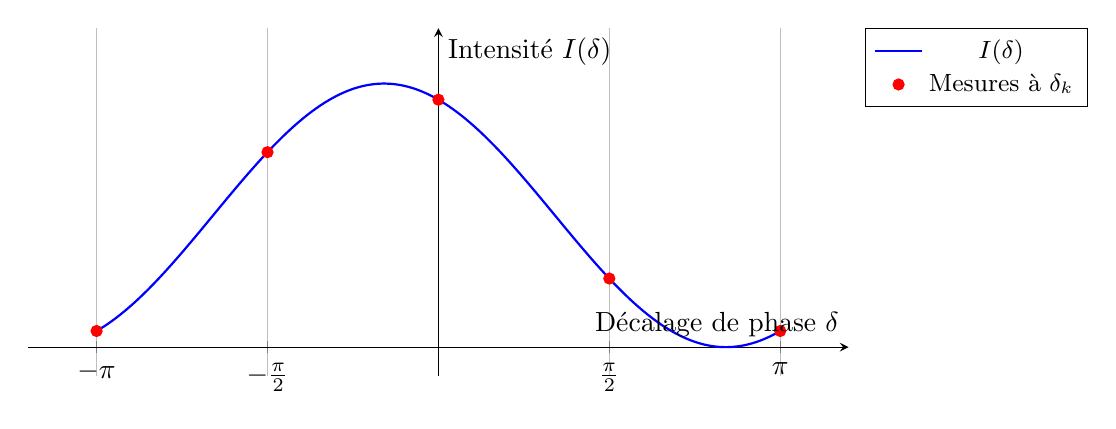
\begin{tikzpicture}
  \begin{axis}[
    domain=-pi:pi,
    samples=300,
    axis lines=middle,
    xlabel={Décalage de phase $\delta$},
    ylabel={Intensité $I(\delta)$},
    xtick={-3.1416, -1.5708, 0, 1.5708, 3.1416},
    xticklabels={$-\pi$, $-\frac{\pi}{2}$, $0$, $\frac{\pi}{2}$, $\pi$},
    ytick=\empty,
    ymin=0, ymax=2.2,
    width=12cm, height=6cm,
    grid=both,
    enlargelimits,
  	legend style={
    		at={(1.02,1)}, anchor=north west,
    		draw=black, fill=white, font=\small
	}
  ]
    % Paramètres de la courbe : I_0 = 1, I_1 = 1, phi = 0.5 rad
    \addplot[blue, thick, domain=-pi:pi] {1 + cos(deg(x + 0.5))};
    \addlegendentry{$I(\delta)$}

    % Points rouges pour les 5 mesures aux décalages multiples de pi/2
    \addplot[only marks, mark=*, red, mark size=2pt]
      coordinates {
        (-pi,   {1 + cos(deg(-pi   + 0.5))})
        (-pi/2, {1 + cos(deg(-pi/2 + 0.5))})
        (0,     {1 + cos(deg(0     + 0.5))})
        (pi/2,  {1 + cos(deg(pi/2  + 0.5))})
        (pi,    {1 + cos(deg(pi    + 0.5))})
      };
    \addlegendentry{Mesures à $\delta_k$}
  \end{axis}
\end{tikzpicture}
\caption{Méthode de décalage de phase à 5 pas avec intervalles de $\pi/2$.}
\end{figure}


\subsection{Reconstruction de la phase}

Prenons cinq images d'interférogrammes $I_1$ à $I_5$ prises aux décalages suivants :
\[
\delta = \{-\pi,\; -\tfrac{\pi}{2},\; 0,\; +\tfrac{\pi}{2},\; +\pi\}.
\]
La phase $\phi$ est alors estimée comme :

\begin{equation}
\phi = \arctan\!\left(
\frac{-2 \bigl(I_2 - I_4\bigr)}
{I_1 - 2I_3 + I_5}
\right)
\end{equation}

\noindent
Cette formule est connue comme l'algorithme de Schwider–Hariharan pour le \textit{5-step $\pi/2$‑shift}.


%%%%%%%%%%%%%%%%%%%%%%%%%%%%%%%%%%%%%%%%%%%%%%%%%%%%%%%%%
%%%%%%%%%%%%%%%%%%%%%%%%%%%%%%%%%%%%%%%%%%%%%%%%%%%%%%%%%
%%%%%%%%%%%%%%%%%%%%%%%%%%%%%%%%%%%%%%%%%%%%%%%%%%%%%%%%%

\newpage
%\pagestyle{empty}

\begin{minipage}[c]{.25\linewidth}
	
\includegraphics[width=4cm]{images/Logo-LEnsE.png}
\end{minipage} \hfill
\begin{minipage}[c]{.4\linewidth}

\begin{center}
\vspace{0.3cm}
{\Large \textsc{Interféromètre de ZYGO}}

\medskip

\textbf{\Large Démarche d'analyse}

\end{center}
\end{minipage}\hfill

%%%%%%%%%%%%%%%%%%%%%%%%%%%%%%%%%%
\section{Démarche d'analyse des interférogrammes}

L'analyse des surfaces ou des aberrations passe par l'acquisition d'images d'interférogrammes par le Zygo, avant une reconstruction de la phase (algorithme de Hariharan) et son déroulement.

A partir de cette phase, il est alors possible d'étudier l'état de surface du système optique à analyser puis de calculer les coefficients de Zernike qui permettent par la suite d'identifier les types d'aberrations présentes dans le système.

\medskip

Les grandes étapes sont décrites succinctement dans la figure suivante :

\begin{tcolorbox}[myboxstyle]
\begin{large}
\begin{center}
L'application se lance par le bouton \textbf{\textsc{Start\_Zygo\_XA.bat}} sur le bureau.
\end{center}
\end{large}
\end{tcolorbox}

\textit{où X est soit 1 (contrôles interférométriques) soit 2 (aberrations).}

\begin{center}
	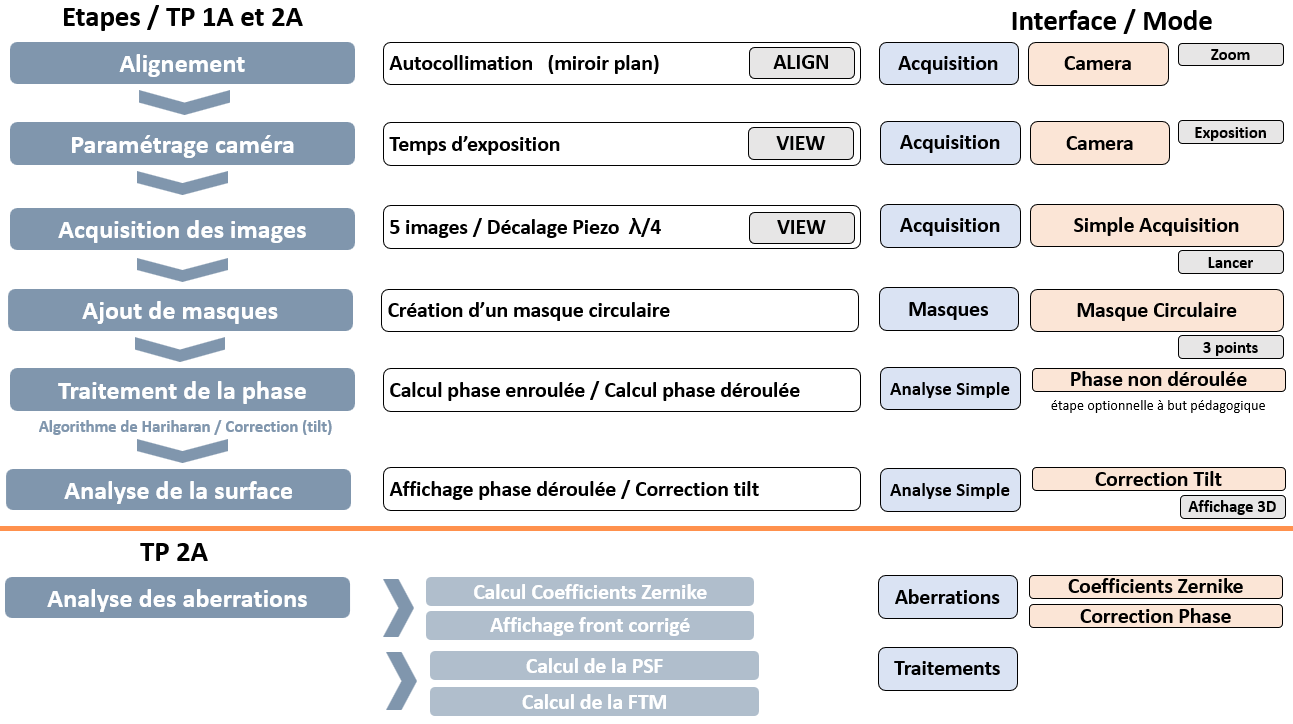
\includegraphics[width=\textwidth]{images/zygo_main_algo.png}
\end{center}

\medskip

Les différents éléments de l'interface de pilotage seront présentés dans la suite de ce document.

\medskip

\medskip

\begin{center}
	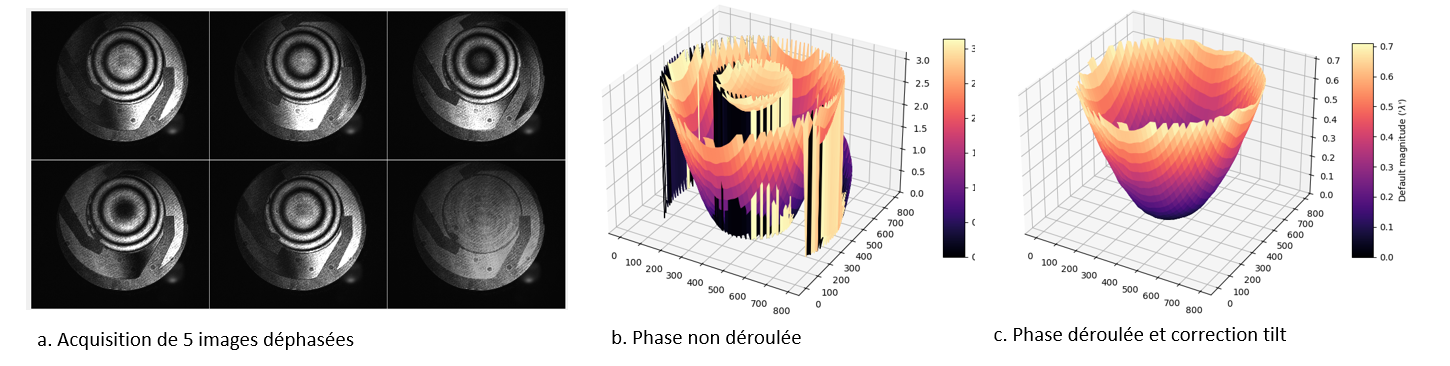
\includegraphics[width=\textwidth]{images/zygo_resultats.png}
\end{center}